
\begin{figure}[t!]
 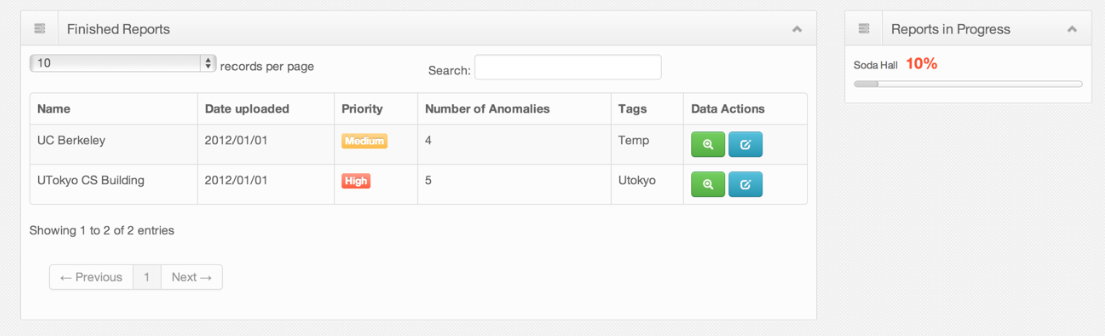
\includegraphics[width=.5\textwidth]{img/eh_alarmlist.png}
 \caption{Screenshot showing a list of alarms found by the Headhunter application, listed in statistically-significant order.}
 \label{fig:ehalarmlist}
\end{figure}

\begin{figure}[t!]
 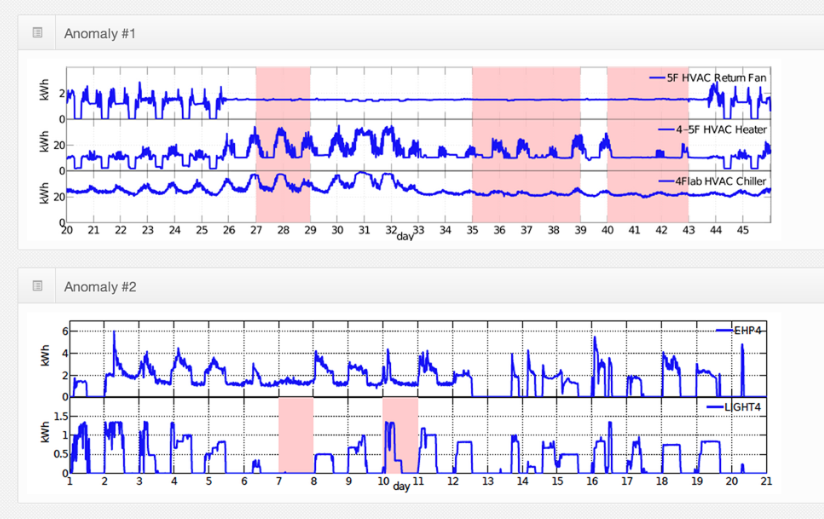
\includegraphics[width=.5\textwidth]{img/eh_screenshot1.png}
 \caption{Screenshot of a portfolio of alarms in the Headhunter application, showing the segments of the traces that triggered an alarm.}
 \label{fig:ehgraphs}
\end{figure}


\section{Demo description}
\label{sec:demo}
We have integrated SBS into a fully functional anomaly detection system for building managers.  The system 
is designed as a web application that takes a bulk-data feed, runs SBS on the data, and displays the associated 
signals where anomalies have been detected.  This system address two challenges that are not addressed in the 
paper~\cite{sbs:ipsn2013}.  It accepts user input on the anomalies that were detected, so that the system can learn
how to distinguish between a potential false-positive and true-positive.  True/false negatives are more difficult
to address because only the building manager can determine them (if they could hypothetically examine all the data).
Secondly, it provides a common vocabulary
to users to help normalize the data across different data sets and buildings.  A \emph{major} challenge in buildings 
is that the vocabulary and inter-relationships between the sensor, spaces, and sub-system varies slightly
from building to building.  By providing a tagging 
mechanism, we attempt to embed semantic information
that can be used to characterize the classes of anomalies and faults found with the SBS tool.